Following the approach in \probref{chapters/11/10/3/12},
\begin{align}
\cos45\degree 
\frac{1}{\sqrt{2}} = \frac{\myvec{2 & 1} \myvec{1\\m}}{\norm{\myvec{2\\1}}\norm{\myvec{1\\m}}}
\\
\implies 
 3m^2 - 8m -3 = 0
 \\
\text{or, }
m= - \frac{1}{3}, 3
\end{align} 
Thus, the desired equations are 
\begin{align}
	\myvec{3&-1}\cbrak{\vec{x}-\myvec{3\\2}}&=0\\
 \implies 	\myvec{3 & -1}\vec{x} &= 7
\end{align}
and 
\begin{align}
	\myvec{1&3}\cbrak{\vec{x}-\myvec{3\\2}}&=0\\
		\implies 	\myvec{1 & 3}\vec{x} &= 9
\end{align}
See
\figref{fig:chapters/11/10/4/11/figs/strline.jpg}.
\begin{figure}[H]
\centering
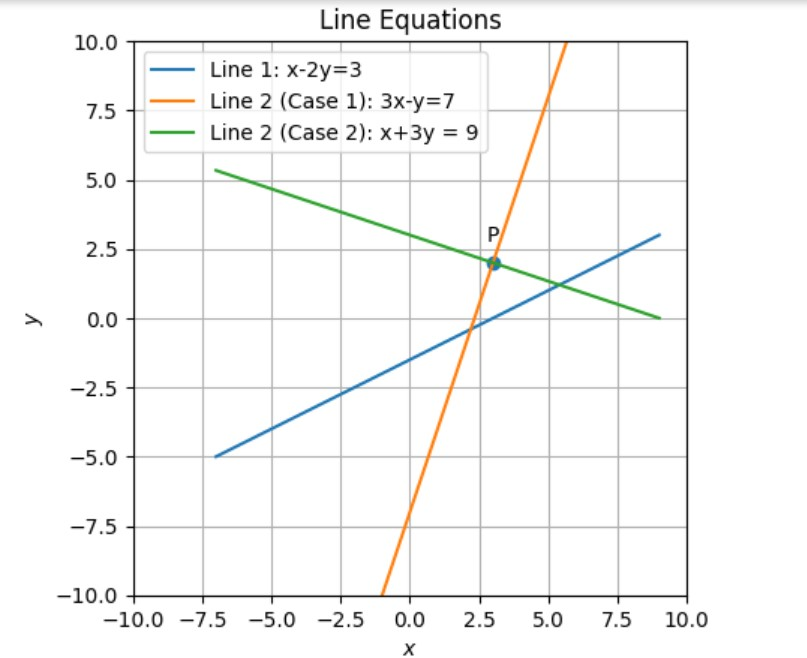
\includegraphics[width=0.75\columnwidth]{chapters/11/10/4/11/figs/strline.jpg}
\caption{}
\label{fig:chapters/11/10/4/11/figs/strline.jpg}
\end{figure}
